% !TEX TS-program = pdflatex

\documentclass[unicode,11pt,notheorems,xcolor=table]{beamer}

\usepackage[T2A]{fontenc}
\usepackage[utf8]{inputenc}
\usepackage[russian]{babel}
\usepackage{amsmath,amsfonts,amssymb,amsthm}
\usepackage{mathtools}
\usepackage{diagbox}

\usepackage{ulem}
\usepackage{tikz, graphicx}
%\usepackage{tkz-graph}
\usetikzlibrary{matrix,arrows,decorations.pathmorphing, arrows.meta,positioning}
\usetikzlibrary{positioning,calc}
\usetikzlibrary{petri}
\usetikzlibrary{decorations.pathreplacing}

%Описание стиля презентации
\usetheme[sidebar=0]{kfmn} 
\setbeamercovered{transparent}

%\definecolor{cyan}{RGB}{240,217,1}
%\definecolor{vgugreen}{RGB}{143,188,103}
%\definecolor{vgured}{RGB}{234,38,40}
%\definecolor{vgublue}{RGB}{53,101,167}



\makeatletter
	\g@addto@macro{\endtabular}{\rowfont{}}% Clear row font
	\makeatother
	\newcommand{\rowfonttype}{}% Current row font
	\newcommand{\rowfont}[1]{% Set current row font
		\gdef\rowfonttype{#1}#1\ignorespaces%
	}
\makeatother

\newcommand{\myunit}{9mm}
\tikzset{
    node style sp/.style={draw,circle,minimum size=\myunit},
    node style ge/.style={circle,minimum size=\myunit},
    arrow style mul/.style={draw,sloped,midway,fill=white},
    arrow style plus/.style={midway,sloped,fill=white},
}

%[0, 6, 8, 8, 10, 5, 6, 10, 8, 10, 10], 

\pgfdeclareimage[height=8mm]{university-logo}{logo-iem.png}
\logo{\pgfuseimage{university-logo}}
%2[0, 11, 10, 8, 11, 5, 11, 11, 8, 11, 10, 11],

\titlepicture{
	\begin{tikzpicture}[y=1.4cm,overlay,rotate=8]
	\coordinate (O) at (-3cm,0.9cm);
	\filldraw[thick,draw= vgublue, fill=vgublue!20!white] (0,0) circle[radius=4.2cm];
	\clip (0,0) circle[radius=4.2cm];
	\draw (-1.5,1.5) node{
	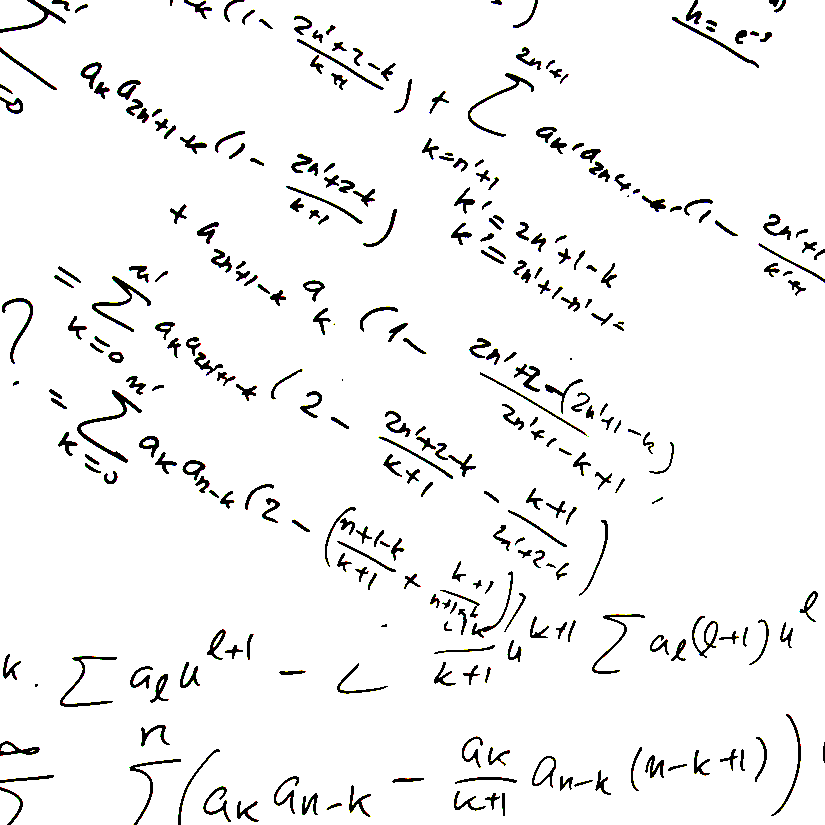
\includegraphics[width=8cm]{titlepic.png}
	};
\end{tikzpicture}
}

\usepackage[math]{iwona}

\newcommand{\hplus}{\mathbin{\hat+}}
\newcommand{\hdot}{\mathbin{\hat\cdot}}
% Описание теорем
\newtheorem{theorem}{Теорема}
\newtheorem{seq}{Следствие}
%%

\LECT % 

% Титульный лист теорем
\author[Д.\,В. Чупраков]{канд.\,физ.-матем.\,наук, доцент Д.\,В. Чупраков\\[6pt] usr10381@vyatsu.ru}

\institute[ВятГУ]{ФГБОУ ВО Вятский государственный университет}

\department{Факультет экономики и финансов}

\title[Лекция~9. Многокритериальные задачи]{
	Введение в экономико-математическое моделирование\\[12pt]
	Лекция~9. Многокритериальные задачи}

\date{2 ноября 2020~г.}


\setbeamercovered{invisible}



\begin{document}


\maketitle

\begin{frame}{Структура лекции}
	\tableofcontents
\end{frame}

\section{Проблема нескольких критериев}
\begin{frame}{Задача многокритериальной оптимизации}
    \begin{itemize}
        \item Имеется область допустимых планов.
        \item Есть несколько целевых функций.
        \item Целевые функции не могут быть совмещены в одну.
    \end{itemize}
    \medskip
    \hrule
    \medskip
    Требуется найти точку области допустимых решений, в которой достигается максимум (или минимум) всех целевых функций. 
\end{frame}
\section{Множество Парето}
\begin{frame}{Оптимальность по Парето}
    \alert{«Всякое изменение, которое никому не приносит убытков, а некоторым людям приносит пользу (по их собственной оценке), является улучшением»}
\end{frame}

\begin{frame}{Множество Парето}
    По отношению Парето некий допустимый \alert{план $X$ лучше плана $Y$} ($X > Y$), если 
    \begin{itemize}
        \item $X$ не хуже, чем $Y$ по каждому из критериев: \alert{$F_i(X) \geqslant F_i(Y)$ для всех $i$};
        \item хотя по одному из критериев $X$ лучше, чем $Y$: \alert{$F_j(X) > F_j(Y)$ для некоторого  $j$}.
    \end{itemize}


    План $X$~--- \alert{Парето-оптимальное решение}, если не существует такого плана $Y$, что $Y > X$ по Парето.

    \alert{Множеством Парето}~--- множество  всех Парето-оптимальных решений задачи.
\end{frame}

\begin{frame}{Выбор Парето-оптимальных альтернатив при решении многокритериальной задачи}

\end{frame}

\begin{frame}{Пример}
    \begin{exampleblock}{}
        Приближенно построить множество Парето-оптимальных альтернатив для следующей задачи двухкритериальной оптимизации:
    
    $$  
    \begin{aligned}
        F_1 &= (x-2)^2+(y-1)^2\\
        F_2 &= (x-5)^2+(y-5)^2\\
    \end{aligned}
        \qquad
        D_X\colon 
        \left\lbrace
        \begin{aligned}
            0 \leqslant &x \leqslant 5\\
            1 \leqslant &y \leqslant 5    
        \end{aligned}
        \right.
    $$
\end{exampleblock}
\end{frame}

\begin{frame}{Пример}
    Покрытие множества сеткой.
    Множество допустимых значений покрытое равномерной сеткой с шагом 1 по обеим осям координат.
\end{frame}
\section{Метод ограничений}

\section{Метод идеальной точки}


\section{Резюме и источники}
\begin{frame}{Резюме}
	Теперь вы знаете:
	\begin{enumerate}
	\item 
		Общую балансовую модель.
	\item 
		Модель Леонтьева.
	\end{enumerate}
	Убедитесь, что вы не только знаете, но и умеете применять рассмотренные методы.
	
	Для успешного применения модели вы должны уметь:
	\begin{itemize}
		\item 
			Умножать матрицы.
		\item 
			Вычислять определители.
		\item 
			Находить обратную матрицу
		\item 
			Проверять матрицу на продуктивность.
		\end{itemize}
	
\end{frame}

\begin{frame}{Источники информации}
\begin{itemize}
\item 
	{\color{blue}\href{https://cloud.mail.ru/public/jWCR/2BBwXTrkg}{Высшая математика для экономистов.}} Под~ред.~Н.\,Ш.~Кремера. Глава~2, \S 2.7 c. 56--60.
\item 
	{\color{blue}\href{https://cloud.mail.ru/public/5c87/4Cmo8H9BA}{Высшая математика для экономистов. Практикум.}} Под~ред.~Н.\,Ш.~Кремера.  \S 2.5 c. 50--55.

\item 
	Все материалы по курсу здесь:
{\color{blue}\url{https://cloud.mail.ru/public/48BX/47oESuaQQ}}
\end{itemize}

\end{frame}

\end{document}
